\documentclass[]{article}
\usepackage{lmodern}
\usepackage{graphicx}
\usepackage{adjustbox}
\usepackage{amssymb,amsmath}
\usepackage{ifxetex,ifluatex}
\usepackage{listings}
\usepackage[T1]{fontenc}
\usepackage[utf8]{inputenc}
\usepackage{microtype}
\usepackage[margin=1in]{geometry}
\usepackage{hyperref}
\usepackage{framed}
\usepackage{graphicx,grffile}
\usepackage{multirow}
\makeatletter
\def\maxwidth{\ifdim\Gin@nat@width>\linewidth\linewidth\else\Gin@nat@width\fi}
\def\maxheight{\ifdim\Gin@nat@height>\textheight\textheight\else\Gin@nat@height\fi}
\makeatother
% Scale images if necessary, so that they will not overflow the page
% margins by default, and it is still possible to overwrite the defaults
% using explicit options in \includegraphics[width, height, ...]{}
\setkeys{Gin}{width=\maxwidth,height=\maxheight,keepaspectratio}
\setlength{\parindent}{0pt}
\setlength{\parskip}{6pt plus 2pt minus 1pt}
\setlength{\emergencystretch}{3em}  % prevent overfull lines
\providecommand{\tightlist}{%
  \setlength{\itemsep}{0pt}\setlength{\parskip}{0pt}}

%%% Change title format to be more compact
\usepackage{titling}

% Create subtitle command for use in maketitle
\newcommand{\subtitle}[1]{
  \posttitle{
    \begin{center}\large#1\end{center}
    }
}

\setlength{\droptitle}{-2em}
  \title{MSAN 621 - Homework 1}
  \pretitle{\vspace{\droptitle}\centering\huge}
  \posttitle{\par}
  \author{Andre Guimaraes Duarte}
  \preauthor{\centering\large\emph}
  \postauthor{\par}
  \predate{\centering\large\emph}
  \postdate{\par}
  \date{October 31, 2016}
  
% Redefines (sub)paragraphs to behave more like section*s
\ifx\paragraph\undefined\else
\let\oldparagraph\paragraph
\renewcommand{\paragraph}[1]{\oldparagraph{#1}\mbox{}}
\fi
\ifx\subparagraph\undefined\else
\let\oldsubparagraph\subparagraph
\renewcommand{\subparagraph}[1]{\oldsubparagraph{#1}\mbox{}}
\fi

\usepackage{color}

%%%%%%%%%%%%%%%%%%%%%%%%%%%%%%%%%%%%%%%%%%%%%%%%%%%%%%%%%%%%%%%%%%%%%%%%%%%%%%%%%%%%%%%%%%%%%%%%%%%%%%%%%%%%%%%%%%%%%%%
\begin{document}
\maketitle

\section{The Boston Data Set}

The models are trained with all data except the last 50 rows, which are reserved to test the models' performance.

For MLR, we get an MSE of 10.967.

For kNN, we get an MSE that varies according to k, as shown in the table below:

\begin{center}
\begin{tabular}{c|c}
k & MSE\\
\hline
1 & 29.299\\
2 & 24.532\\
3 & 22.003\\
4 & 25.754\\
5 & 26.200\\
6 & 24.441\\
7 & 24.615\\
8 & 22.820\\
9 & 24.117\\
10 & 22.371\\
11 & 23.036\\
12 & 24.953\\
13 & 23.774\\
14 & 24.388\\
15 & 27.162\\
16 & 25.311\\
17 & 24.743\\
18 & 25.761\\
19 & 27.539\\
20 & 27.362\\
\end{tabular}
\end{center}

Plotting MSE against k for both models, we get the image below:

\begin{center}
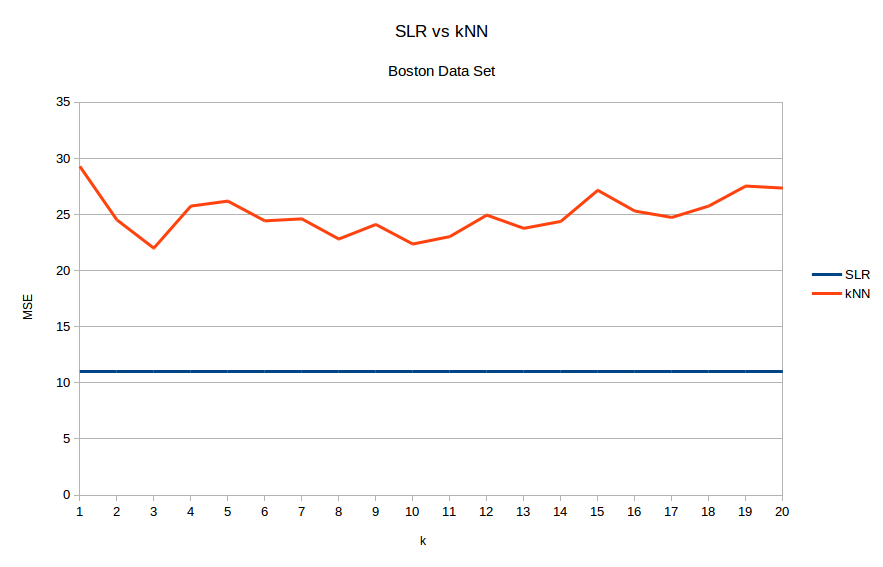
\includegraphics[width=\linewidth]{boston.png}
\end{center}

We can see that we get a lower test MSE with SLR than kNN, for any value of k. For this example, simple linear regression is a better algorithm for predicting new data from the Boston Data Set.

\section{The U.S. Monthly Climate Normals Data Set}
The models contain daily and hourly temperature for a year from 457 weather stations across the US. The models are trained on the data from all stations except 1-5 that are used for testing and assessing the models' performance. The results are shown in the table below, where $n$ is the number of test stations used.

\begin{center}
\begin{tabular}{c|c|c|c|c|c|c}
Model & k & MSE (n=5) & MSE (n=4) & MSE (n=3) & MSE (n=2) & MSE (n=1)\\
\hline
MLR & - & 7.030 & 7.633 & 7.204 & 8.936 & 1.487\\
\hline
\multirow{20}{*}{kNN}
& 1 & 114.261 & 19.209 & 21.026 & 35.079 & 23.071\\
& 2 & 48.180 & 18.735 & 16.955 & 30.678 & 16.610\\
& 3 & 31.858 & 15.543 & 16.519 & 29.068 & 14.960\\
& 4 & 25.050 & 14.476 & 15.247 & 89.643 & 13.897\\
& 5 & 20.884 & 13.710 & 14.570 & 74.330 & 13.181\\
& 6 & 19.201 & 13.186 & 14.286 & 61.624 & 12.916\\
& 7 & 17.446 & 12.722 & 14.196 & 52.829 & 12.718\\
& 8 & 16.096 & 12.376 & 14.295 & 46.494 & 12.468\\
& 9 & 15.664 & 12.242 & 14.100 & 42.343 & 12.223\\
& 10 & 15.085 & 12.043 & 13.870 & 39.005 & 12.017\\
& 11 & 14.454 & 11.904 & 13.689 & 36.140 & 11.854\\
& 12 & 14.103 & 11.792 & 13.725 & 34.312 & 11.807\\
& 13 & 13.717 & 11.769 & 13.635 & 32.643 & 11.769\\
& 14 & 13.412 & 11.778 & 13.542 & 31.180 & 11.682\\
& 15 & 13.172 & 11.910 & 13.504 & 30.002 & 11.605\\
& 16 & 12.917 & 11.870 & 13.589 & 29.278 & 11.507\\
& 17 & 12.748 & 11.820 & 13.631 & 28.626 & 11.437\\
& 18 & 12.729 & 11.737 & 13.551 & 27.968 & 11.331\\
& 19 & 12.846 & 11.766 & 13.593 & 27.464 & 11.250\\
& 20 & 12.807 & 11.790 & 13.534 & 27.141 & 11.208\\
\end{tabular}
\end{center}

Fixing $k=3$, we can get results for each station individually and for all five combined. The MSEs are reported in the table below.

\begin{center}
\begin{tabular}{c|c|c|c|c|c|c}
\multirow{2}{*}{Model} & MSE & MSE & MSE & MSE & MSE & MSE\\
& (USW00023234) & (USW00014918) & (USW00012919) & (USW00013743) & (USW00025309) & (all 5)\\
\hline
MLR & 1.487 & 16.374 & 3.731 & 8.914 & 4.604 & 7.030 \\
kNN & 14.960 & 108.360 & 30.754 & 13.052 & 21.473 & 31.858 \\
\end{tabular}
\end{center}

We can see that MLR performs better (i.e., produces a lower MSE) than kNN for this data set. In addition, the prediction produced vary depending on the test set used. For example, predictions for station \texttt{USW00014918} are considerably worse than those for station \texttt{USW00023234}

The imputer strategy used for this model is very basic: missing/erroneous values are replaced with the mean temperature observed across all stations, days, and hours. Although this strategy may be suited in some cases, I don't think that it makes much sense here. Stations can be located in places where the climate is very different, so the mean temperature across the country and the year may not fit well in those missing places. In order to improve this, we could think about imputing missing readings with the average temperature throughout the year for that station, or even more locally (i.e., for that month for example) if data is available.

In general, MLR performed better than kNN, at least for $k$ up to 20. In particular, the MSE for MLR when 5 stations are used for the test data is very low ($1.487$). The performance of MLR for this dataset is impressive.

I think it would be interesting to explore different imputing strategies to see how this affects the models' performance. The tactic used here is very basic, so improvement is definitely possible in this area. However, I think the results obtained thus far are very good already. Other features may be used to get even lower MSEs: for instance, we may want to get geographical information about the weather stations in order to group them by climate and overall weather patterns to get better averages.


\end{document}
